% =====================================================================
\chapter{Termo dominante e análise assintótica}\label{cap:04}
\naaula{17 a 19}

No capítulo 2, a soma de um vetor custou $3n + 4$ passos, e os laços aninhados custaram
$3n^2 + 4n + 2$. Essas fórmulas são exatas, mas têm detalhes demais. Neste capítulo você vai
aprender a ficar só com o que importa.

\section{Quem manda quando \texorpdfstring{$n$}{n} cresce}

Tome $T(n) = 3n^2 + 5n + 2$ e veja quanto cada termo contribui para o total:

\begin{center}
\begin{tabularx}{\textwidth}{L C C C C}
\cab \tcx{$n$} & \tcx{$3n^2$} & \tcx{$5n$} & \tc{2} & \tcx{PARTE DE $3n^2$ NO TOTAL} \\
10 & 300 & 50 & 2 & 85,2\% \\
\rowcolor{edfundo} 100 & 30.000 & 500 & 2 & 98,4\% \\
1.000 & 3.000.000 & 5.000 & 2 & 99,8\% \\
\rowcolor{edfundo} 1.000.000 & $3 \times 10^{12}$ & $5 \times 10^{6}$ & 2 & 99,9998\% \\
\end{tabularx}
\end{center}

\begin{figure}[!htb]
  \centering
  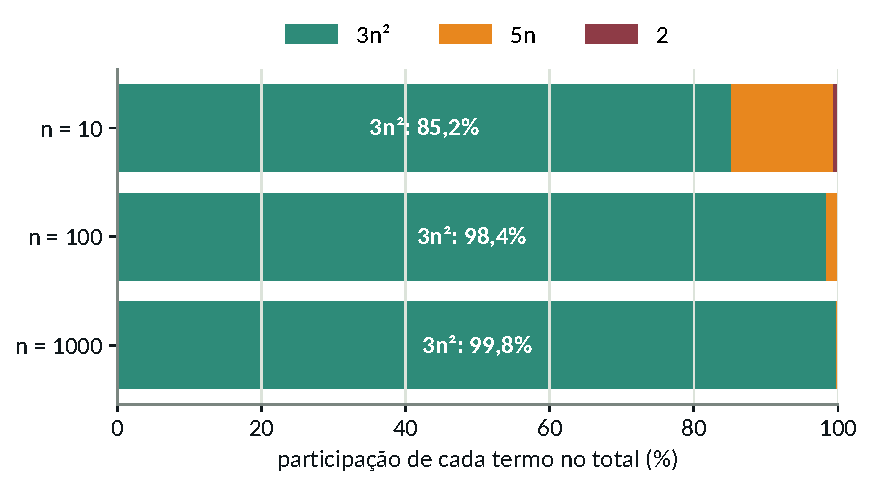
\includegraphics[width=0.74\textwidth]{figuras/f04_termo_dominante.pdf}
  \caption{Quanto maior $n$, mais o termo $3n^2$ domina o total.}
\end{figure}

O termo que cresce mais rápido — aqui, $3n^2$ — acaba respondendo por praticamente todo o custo.
Ele é chamado de \textbf{termo dominante}. Os outros ficam cada vez mais irrelevantes.

\begin{intuicao}
É como comprar um carro e um cafezinho: o preço total é \enquote{o preço do carro}. Ninguém
deixa de comprar o carro por causa do cafezinho. Em $3n^2 + 5n + 2$, o $3n^2$ é o carro.
\end{intuicao}

\section{As duas regras de simplificação}

\begin{enumerate}
  \item \textbf{Fique só com o termo dominante:} $3n^2 + 5n + 2 \;\to\; 3n^2$.
  \item \textbf{Despreze a constante que multiplica:} $3n^2 \;\to\; n^2$.
\end{enumerate}

Dizemos então que $T(n)$ \enquote{cresce como $n^2$}, ou que ele é \enquote{quadrático}.

Por que podemos desprezar a constante? Lembre do capítulo 1: rodar o mesmo algoritmo numa máquina
mais lenta, ou em Python em vez de C, multiplica o tempo por uma constante (ali, cerca de 35).
Constantes mudam de máquina para máquina; a \textbf{forma do crescimento} não muda. Como queremos
uma medida que valha em qualquer máquina, deixamos a constante de lado.

\begin{center}
\begin{tabularx}{0.9\textwidth}{L L L}
\cab \tc{Custo exato} & \tc{Termo dominante} & \tc{Cresce como} \\
$3n + 4$ & $3n$ & $n$ \\
\rowcolor{edfundo} $3n^2 + 4n + 2$ & $3n^2$ & $n^2$ \\
$2\log_2 n + 2$ & $2 \log_2 n$ & $\log n$ \\
\rowcolor{edfundo} $\dfrac{n(n-1)}{2} = \dfrac{n^2}{2} - \dfrac{n}{2}$ & $\dfrac{n^2}{2}$ & $n^2$ \\
$2^n + n^3$ & $2^n$ & $2^n$ \\
\rowcolor{edfundo} $500$ & $500$ & constante \\
\end{tabularx}
\end{center}

\begin{atencao}
Para achar o termo dominante, use a hierarquia do capítulo 3: uma constante cresce menos que
$\log n$, que cresce menos que $n$, que cresce menos que $n^2$, que cresce menos que $2^n$, que
cresce menos que $n!$. Na dúvida, calcule os termos para um $n$ grande, como $n = 1.000$.
\end{atencao}

\section{Análise assintótica}

\textbf{Análise assintótica} é o nome técnico de \enquote{olhar o comportamento quando $n$ fica
muito grande}. A palavra vem de \emph{assíntota}, uma linha da qual uma curva se aproxima cada
vez mais.

Veja por que isso importa. Imagine dois algoritmos: $A$, que faz $100n$ passos, e $B$, que faz
$n^2$. Para $n = 10$, $A$ faz 1.000 passos e $B$ só 100: $B$ parece melhor! Mas:

\begin{figure}[!htb]
  \centering
  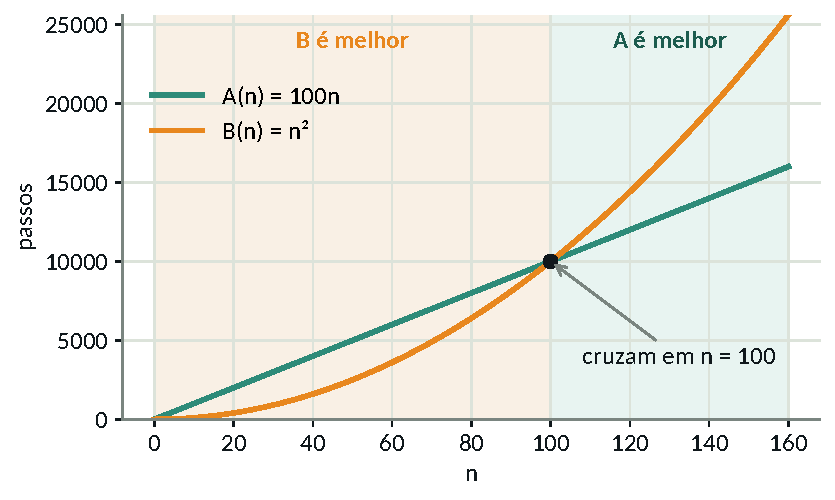
\includegraphics[width=0.72\textwidth]{figuras/f04_cruzamento.pdf}
  \caption{$100n$ e $n^2$ se cruzam em $n = 100$. Depois disso, $A$ ganha, e a vantagem só aumenta.}
\end{figure}

\begin{center}
\begin{tabularx}{\textwidth}{P{2.8cm} C C C C}
\cab \tcx{$n$} & \tc{10} & \tc{100} & \tc{1.000} & \tc{1.000.000} \\
$A(n) = 100n$ & 1.000 & 10.000 & 100.000 & $10^8$ \\
\rowcolor{edfundo} $B(n) = n^2$ & 100 & 10.000 & 1.000.000 & $10^{12}$ \\
\end{tabularx}
\end{center}

Para um milhão de elementos, $B$ faz \textbf{dez mil vezes} mais trabalho que $A$. A constante 100
de $A$ assustava no começo, mas perdeu completamente a importância. Por isso comparamos
algoritmos pela forma do crescimento: \textbf{para $n$ grande, quem cresce mais devagar sempre
vence}, qualquer que seja a constante.

\section{Um cuidado: desprezar não é ignorar sempre}

A análise assintótica fala de $n$ grande. Para entradas pequenas, as constantes podem, sim,
decidir quem é mais rápido. É por isso que bibliotecas reais combinam algoritmos: o
\codigo{sort()} do Python, por exemplo, usa um algoritmo \enquote{de família menor} para listas
grandes, mas troca para o Insertion Sort (capítulo 9) em trechos pequenos, onde ele é mais
rápido na prática.

\begin{exrapido}
Diga como cresce cada função: (a) $4n + 10$; (b) $\dfrac{n^2}{2} + 3n$; (c) $5 + 2\log_2 n$;
(d) $2^n + n^3$; (e) $1.000$. Depois: com $A(n) = 50n$ e $B(n) = n^2$, a partir de qual $n$ o
algoritmo $A$ passa a ser melhor?
\end{exrapido}

\begin{respostas}
  \resp{4.1} (a) como $n$; (b) como $n^2$; (c) como $\log n$; (d) como $2^n$; (e) é constante.
  Os dois se igualam quando $50n = n^2$, isto é, em $n = 50$. Para $n > 50$, $A$ é melhor.
\end{respostas}
